\chapter{Introduzione}
\begin{comment}
con il problema e l'idea non ci siamp proprio..
la scaletta dei capitoli è:
- introduzione
- stato dell'arte
- metodi e strumenti
- sviluppo del progetto
- risultati

Sottosezioni di introduzione:
- Motivaione

    - modelli neurali per la segmentazione dei difetti
        - applicazioni
        - il dataset e i requisiti per l'addestramento

- Approccio al problema

    - La generazione di un dataset sintetico

- introduzione alle reti neurali

    - feedforward networks
        - il neurone
        - la funzione di attivazione
        - backpropagation

    - convolutional neural networks
        - la convoluzione
        - il pooling
        - l'upsampling

\end{comment}


\section{Motivaione \ok}
\begin{comment}
\end{comment}

\subsection{Modelli neurali per la segmentazione nel contorllo qualità\ok}
\begin{comment}
    Done.
\end{comment}

Oggi le reti neurali trovano un vasto impiego in moltissi campi, dall'industria alla medicina, fino alla vita di tutti i giorni.
Il grande vantaggio che ci portano è la capacità di apprendere da un set di dati, e di generalizzare su di uno nuovo,
permettendocci di risolvere problemi che altrimenti sarebbero matematicamente troppo complessi da risolvere con un algoritmo.
Ci sono vari esempi in cui i modelli neurali raggiungono risultati superiori a quelli ottenuti dall'uomo, in determinati task, 
o almeno se non lo superano in termini di accuratezza, lo fanno in termini di velocità, scalabilità, costi e prestazioni.

Un task in cui le reti neurali eccellono è la segmentazione di immagini, ovvero la classificazione pixel per pixel di un'immagine,
questo tipo di task è utilizzato ad esempio nel campo medico per la segmentazione di organi, tumori, o in campo industriale per la segmentazione di difetti,
per la verifica automatica della qualità di un prodotto o di un semilavorato.

Nel caso specifico, per la segmentazione dei difetti l'utilizzo di questo tipo di modelli è molto diffuso, in quanto risolve un grave problema 
che affligge i reparti controllo qualità delle aziende, ovvero il calo della concentrazione al quale un operatore è soggetto dopo un certo numero di ore di lavoro.
Infatti una persona per quanto allenata e preparata, dopo un certo numero di ore di lavoro, è soggetta a stanchezza e con essa
la sua accuratezza nel riconoscere un difetto diminuisce, mentre un modello neurale adeguatamente addestrato, in condizioni ambientli stabili,
come ad esempio una adeguata illuminazione, una videocamera ad alta risoluzione e un'adeguata distanza dal soggetto, sarà in grado di mantenere 
un'accuratezza costante, senza necessità di fermarsi per riposare. Questo si traduce in un risparmio di tempo e di denaro per l'azienda,
In quanto il controllo manuale richiede più tempo ed è più soggetto ad errori, i quali spesso si trasformano in ritardi nella consegna dei prodotti,
spese di trasposrto aggiuntive per il ritorno o la sostituzione del prodotto, o addirittura la perdita di un cliente.

\begin{figure}[H]
    \centering
    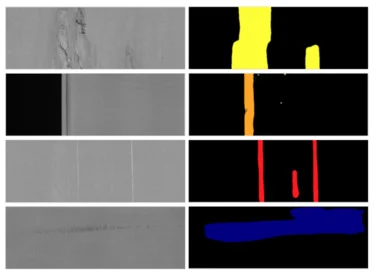
\includegraphics[width=0.4\textwidth]{imgs/segm_example_1_crop.png}
    \caption{An example of segmented defects from the "Severstal steel defect dataset".
    credits: Neven Robby and Goedemé Toon, 2021, A Multi-Branch U-Net for Steel Surface Defect Type and Severity Segmentation.
    https://www.mdpi.com/2075-4701/11/6/870}
    \label{fig:segm_example_1}
\end{figure}


\subsection{Il dataset, requisiti e problematiche di realizzazione \ok}
\begin{comment}
    Va rivisto il contenuto e integrate le parti provenienti dalla sezione precedente.
\end{comment}

La problematica di avere un modello con elevata accuratezza per task di segmentazione è relativa alla quantità e qualità dei dati necessari,
i quali raramente sono disponibili opensource o per l'acquisto, rendendo necessaria la creazione di un dataset apposito.
Molti task richiedono un grande quantità di dati per essere generalizzati correttamente, e ogni signolo esempio richiede molta concentrazione
da parte dell'annotatore in quanto non sempre i difetti sono ben visibili. 

In generale la creazione di un dataset è un'operazione molto complessa, non solo dal punto di vista dell'annotatore, ma in oltre da un punto di vista
organizzativo e logistico. Infatti ci sono diversi step che si devono seguire:
\begin{itemize}
    \item \textbf{Acquisizione delle immagini}: Le immagini devono essere acquisite in modo da avere una buona qualità, o almeno sufficiente ai fini dell'apprendimento.
        Se possibile in oltre dovrebbero avere una adeguata uniformità di condizioni (luce, distanza, ...) per garantire le migliori prestazioni da parte del modello,
        ovviamente solo se poi è possibile garantire le stesse condizioni anche nell'utilizzo finale del modello, altrimenti una grande varietà delle condizioni
        è preferibile.
    \item \textbf{Definizione delle classi}: Nel caso di dataset multiclasse, uno step molto importnate è quello di scegliere accuratamente le classi
        e definire in maniera univoca l'associazione tra una classe e una particolare tipologia di difetto. Questo passaggio potrebbe sembrare banale ma in realtà
        nasconde delle grandi insidie, infatti una classificazione non adeguata andrà a causare confusione nel modello, diminuendo la sua accuratezza e/o 
        rendendo il lavoro più difficile per gli annotatori andando a rallentare il processo di annotazione o comunque a ridurne la qualità.
        Questo tipo di prolematiche purtroppo si manifestano chiaramente soltanto in uno stato avanzato del progetto,
        rendendo necessarie revisioni della documentazione, modifica di tutti gli esempi già annotati, con conseguente perdita di tempo e denaro.
    \item \textbf{Definizione della documentazione}: Questo passaggio è un'estensione del precedente, e consiste nella definizione di una documentazione
        Che specifichi senza ambiguità, ad un nuovo annotatore come riconoscere senza dubbio un difetto e classificarlo nella giusta classe.
        Questa fase spesso non termina prima dell'inizio dell'annotazione, ma si protrae per tutta la durata del progetto, in quanto
        spesso nuovi casi non previsti si presentano durante l'annotazione, e la documentazione deve essere aggiornata in tempo reale.
    \item \textbf{Annotazione}: Questo è il passaggio più lungo e costoso, in quanto richiede una squadra di persone,
        che devono essere formate per lo specifico task, e che devono essere costantemente seguite per garantire la qualità del lavoro.
    \item \textbf{Revisione}: Assieme all'annotazione questo è un passaggio chiave, in quanto permette di verificare che l'annotazione sia stata fatta correttamente,
        e che non ci siano errori nell'annotazione. Spesso infatti gli annotatori aqcuisicono dei bias errati nei confronti di una certa classe, o di un certo tipo di difetto, 
        che deve essere identificato e reso noto all'annotatore per correggerlo, ed evitare che questo errore si ripeta in futuro.
        Per evitare che ciò accada oltre al primo annotatore lo stesso esempio viene solitamente rivisto da 2 o 4 persone diverse.
        Si noti che gli errori degli annotatori che non vengono identificati verranno appresi dal modello finale come una corretta classificazione, ciò giustifica un tale 
        dispendio di risorse in questa fase.
\end{itemize}

\subsection{Approccio al problema \ok}
\begin{comment}
Realizzare un architettura in grado di generare un buona quantità di dati annotati a partire da una quantità ridotta.
TODO: aggiungi paper di tecnica copy paste
\end{comment}

La creazione di un dataset come precedentemente illustrato è un processo complesso e dispendioso, che richiede molte risorse umane e finanziarie,
dunque l'intento in questo progetto è quello di proporre un approccio alternativo che sia in grado di ridurre per quanto possibile la durata e il costo
di questo lavoro.
Partendo dal presupposto che almeno in parte il dataset deve essere realizzato manualmente, la proposta è quella di realizzare una certa 
quantità di campioni manualmente seguendo lo schema già visto, per poi addestrare un modello neurale per generare ulteriori esempi sintetici,
raggiungendo un numero di esempi totali che permetta di addestrare un modello con buone prestazioni, ad un costo ridotto rispetto al caso in cui
tutti i dati fossero stati realizzati manualmente.

Per la definizione della pipeline di generazione dei dati, si è partiti dal concetto di \textit{generative adversarial network} (GAN), che è un approccio di machine learning
che permette di generare dati sintetici utilizzando come base dati reali, tali dati sintetici possono essere utilizzati per addestrare un modello neurale.
Tale tecnica ha trovato riscontri positivi in molte ricerche pubblicate in ambito di computer vision \cite{ganbasedaugexample}, in cui i modelli gan vengono
utilizzati per espandere il numero di immagini presenti in un dataset e migliorare la generalizzazione di un modello di classificazione.
Ovviamente gli aumenti di accuratezza, precisione e recall dipendono dal numero di esempi presenti nel dataset e dalla complessità del problema.
Tale tecnica potrebbe essere considerata una versione più sofisticata di data augmentation, in quanto permette di generare dati sintetici molto più complessi
e realistici di quelli che si possono ottenere con semplici trasformazioni geometriche o matematiche.
% TODO: a questo punto introduci il problema della segmentazione e come si può risolvere con la tecnica copy paste,
Per generare dati utilizzabili per addestrare un modello di segmentazione però è necessario risolvere un'ulteriore problema,
infatti un normale modello GAN, fedele alla sua definizione originale \cite{goodfellow2014generative}, è in grado di generare intere immagini,
che possono essere utilizzate per addestrare un modello di classificazione, ma non sono utilizzabili per addestrare un modello di segmentazione,
in quanto per l'addestramento di tale architettura è necessario che gli oggetti di interesse abbiano una maschera che specifichi la loro posizione.
Per risolvere questo problema ci sono 2 principali strade illustrate di seguito.

\subsubsection{Generatore con architettura a solo decoder}

    Questo approccio prvede un'architettura a solo decoder, dunque con in ingresso,
    un vettore casuale di dimensione arbitraria, e in uscita un tensore che può contenere i canali rgb di un'imagine e altri n canali per la maschere che
    identificano le classi desiderate.
    Un'esempio di tale architettura a solo decoder potrebbe essere quella di DCGAN \cite{radford2016unsupervised}, illustrata qui sotto.

    \begin{figure}[H]
        \centering
        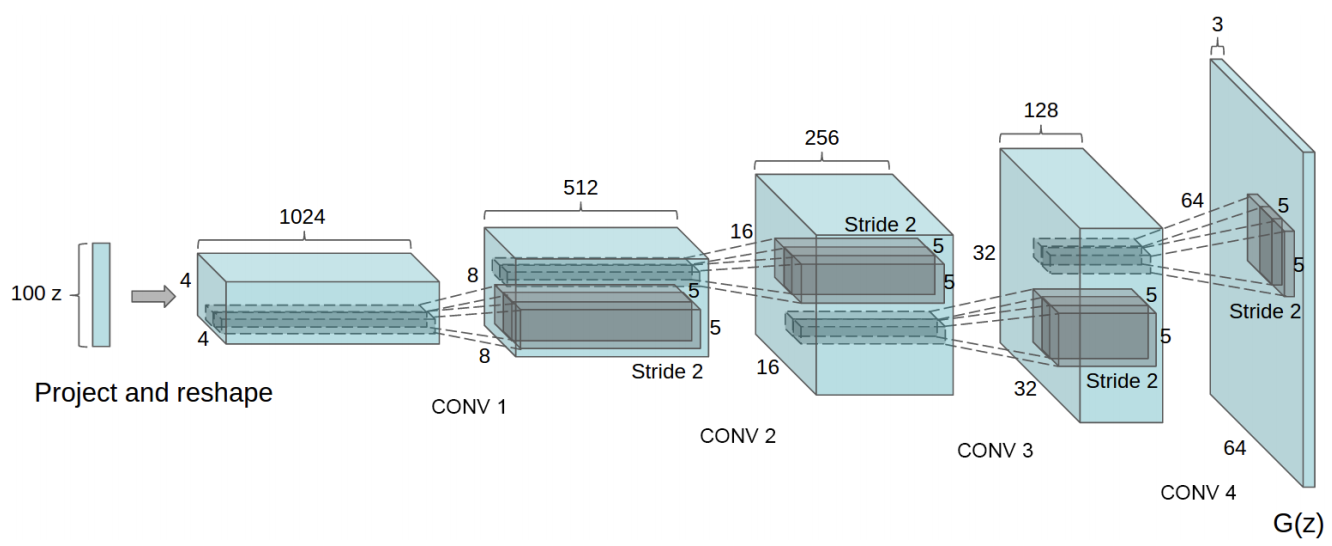
\includegraphics[width=1.0\textwidth]{imgs/DCGAN_architecture_crop.png}
        \caption{Architettura di DCGAN, un esempio di GAN convoluzionale, con architettura a solo decoder.
        credits: Imagine presa dall'articolo di Alec Radford, Luke Metz, Soumith Chintala,
        Unsupervised Representation Learning with Deep Convolutional Generative Adversarial Networks}
        \label{fig:dcgan_architecture}
    \end{figure}

    Questo approccio risulta più semplice da implementare, lasciando però al modello il compito di imparare a generare correttamente
    le immagini e delle maschere coerenti, compito non facile che probabilmente necessita di un elevato numero di esempi. 
    Questa architettura dovrà imparare oltre alla struttura degli oggetti target, a posizionarli nell'immagine.
    Un'altra probblematica di questo approccio è il controllo, infatti l'unico modo di interagire con tale modello è modificando il valore
    del vettore z, il quale permette di spostarsi nello spazio latente, al quale il modello associa diverse caratteristiche dell'immagine
    di output in maniera altamente non lineare, rendendo un eventuale controllo dell'output del modelo molto difficile.
    La difficoltà di controllare il modello rende dunque difficoltoso o impossibile controllare, qualora fosse necessario, la posizione, l'intensità,
    la dimensione o la forma degli oggetti generati.

\subsubsection{Generatore con architettura a encoder-decoder}
    
        

\subsubsection{OLD}
% TODO: passa al caso specifico delle malformazioni e dei difetti introducendo il problema degli artifact dovuti al copy paste in tale caso specifico
% TODO: proponi la soluzione di utilizzare un modello generativo per generare esempi sintetici, con struttura COIGAN.

Per quanto riguarda la segmentazione, l'approccio standard è ..
\begin{comment}
 come vorrei continuare:
    - l'approccio standard per l'augmentation di esempi per la segmentazione è quello del copy paste (cit paper), che permette di 
    generare nuovi esempi partendo da una raccolta di oggetti segmentati e da un dataset di immagini reali senza oggetti, o comunque con dello spazio disponibile
    per poter applicare questi oggetti su tale immagine, effettuando un masking dell'oggetto e applicandolo all'immagine.
    - probblematiche del copy paste: sono relative alla qualità dell'esempio in casi in cui la linea di separazione risulta particolarmente evidente
    può rendere l'esempio non realistico, e potenzialmente spingendo il modello ad associare la segmentazione alla linea di separazione tra oggetto 
    e sfondo, piuttosto che all'oggetto stesso.

\end{comment}


% OLD ####################################################
L'obbiettivo di questo progetto è proporre una soluzione a questo problema, o almeno mitigare la sua gravità.
Per far ciò si propone di realizzare un architettura in grado di generare un oggetto in un'immagine presistente, specificando la maschera di quest'ultimo.

Tale architettura deve essere in grado di prendere in input un'immagine e una maschera, e generare l'oggetto all'interno della maschera, 
lasciando il più possibile invariata l'immagine al di fuori dell'area d'interesse.
Il modello dovrebbe essere in grado di generare un oggetto all'interno dell'area obbiettivo seguendo la distribuzione morfologica degli oggetti 
presenti nel dataset di addestramento.

Tale tecnica è principalmente pensata per tutti quei casi in cui non è semplice o possibile realizzare sinteticamente un oggetto a partire da metodi deterministici, 
ad esempio per la segmentazione dei difetti, i quali non possono essere copiati e incollati in una nuova immagine senza che sia presente un evidente linea di separazione
tra il difetto e il resto dell'immagine, e quindi non possono essere generati con una tecnica di tipo copy paste, senza introdurre artefatti, che potrebbero 
portare ad un peggioramento delle prestazioni del modello, in quanto questo associerebbe il difetto alla linea di separazione.

In questo progetto il dataset utilizzato è Severstal steel defect detection, il quale presenta campioni di acciaio più tosto simili,
ma in generale questa tecnica potrebbe essere utilizzata anche per casi più complessi come il rilevmento di danni su veicoli o edifici,
dove la morfologia del difetto è comune, ma la morfologia, il colore e la texture dell'oggetto su cui deve essere applicato sono differenti 
dal dataset di addestramento, in quest'ultimo scenario infatti non è possibile utilizzare una tecnica di tipo copy paste, in quanto il difetto 
non potrebbe essere applicato in modo coerente con l'immagine base.